\indent Acorde a lo solicitado, mostraremos distintos tipos de familias de casos para nuestro algoritmo, y adem\'as, daremos el tiempo estimado 
seg\'un la complejidad del algoritmo calculada anteriormente.\\

A continuaci\'on mostraremos un gr\'afico de tiempos comparativo entre distintas familias de casos:\\ 

\vspace*{0.3cm} \vspace*{0.3cm}
  \begin{center}
 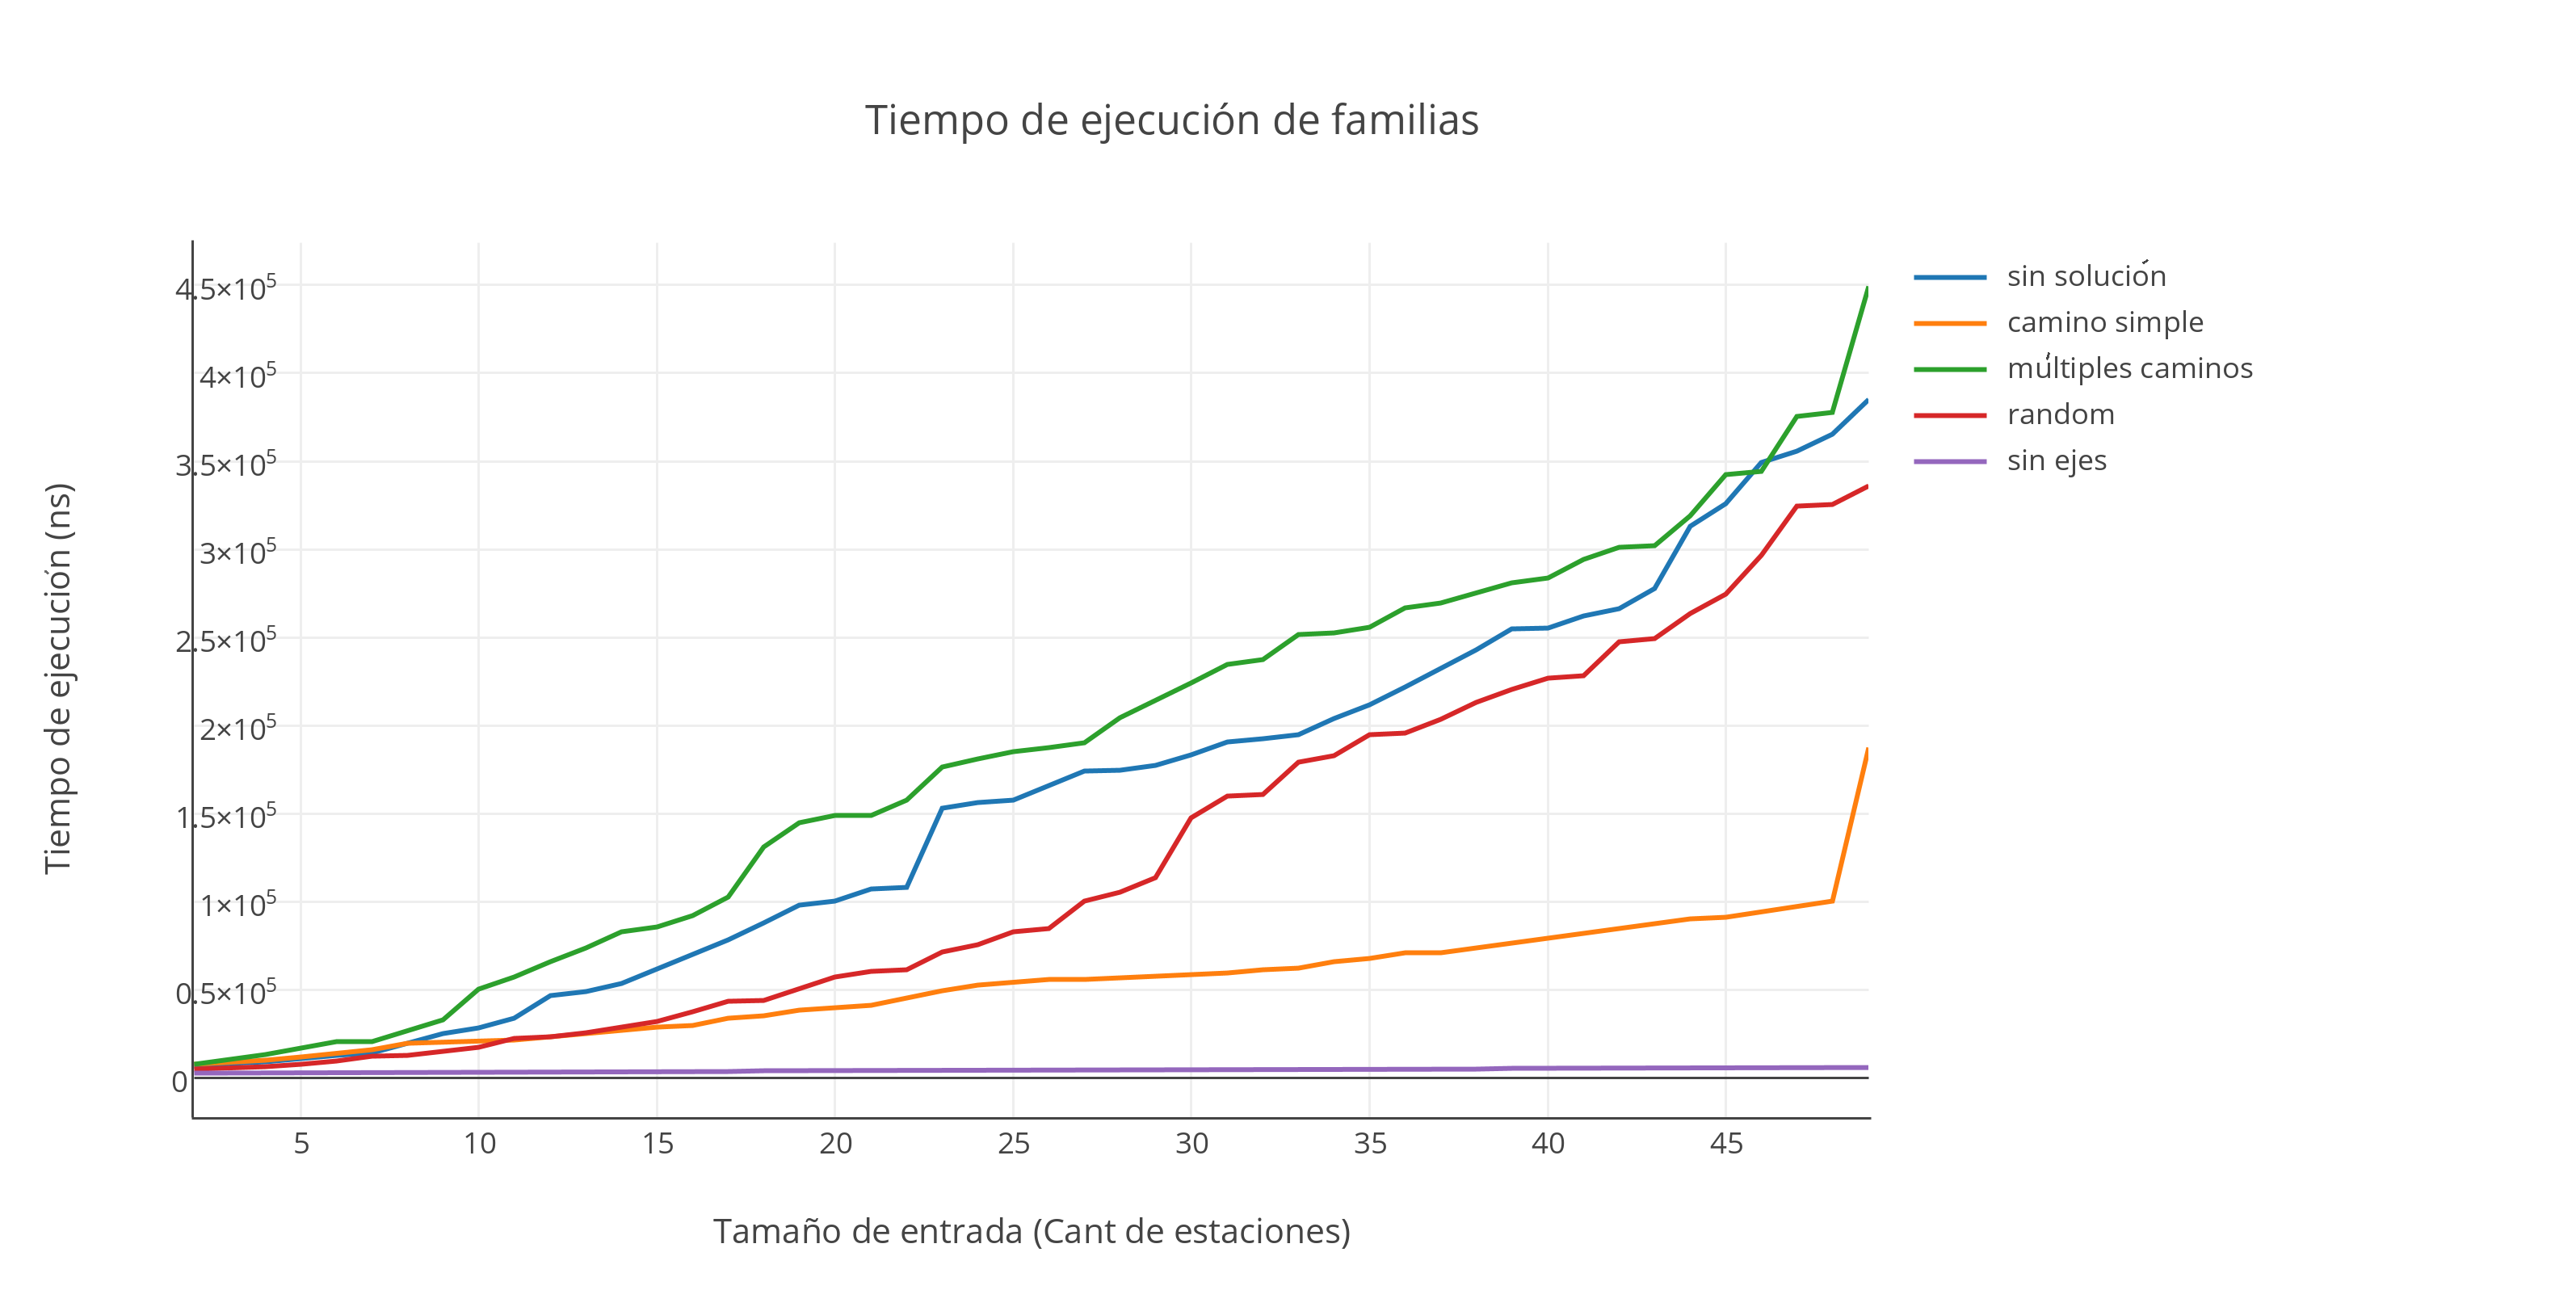
\includegraphics[scale=0.65]{./EJ3/comparativo.png}
 {$Gr$\'a$fico$ \ 3.1 - $Comparativo$}
  \end{center}
  \vspace*{0.3cm}
  
Se puede observar en el gr\'afico, cinco funciones las cuales representan el tiempo de ejecuci\'on de las familias de casos:\\
\begin{itemize}
\item Sin solución
\item Sin ejes
\item Camino simple
\item Múltiples caminos de igual peso llegan a destino
\item Random
\end{itemize}

Como se observa en el gr\'afico la funci\'on representativa de la familia n\'umero 2, presenta una mejor performance en relaci\'on a las otras. Esto se debe a que nuestro algoritmo intenta chequear las aristas para armar los caminos y como encuentra que no hay ningun camino de ningun nodo hacia otro finaliza su ejecuci\'on demandando unicamente la creaci\'on del grafo.

Luego de chequear dichas instancias, pudimos llegar a la conclusi\'on que la familia de casos que presenta una mejor performance para nuestro algoritmo
es en el cual \textbf{No hay ejes, todos los nodos desconectados}

Un grafo representativo de lo dicho ser\'ia el siguiente:

\vspace*{0.3cm} \vspace*{0.3cm}
  \begin{center}
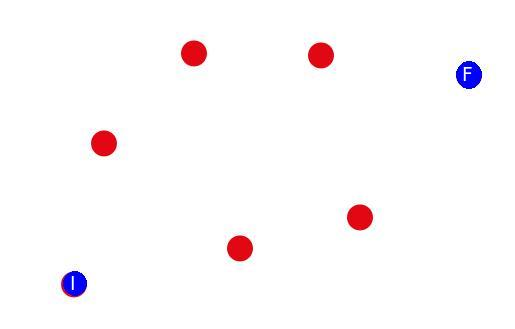
\includegraphics[scale=0.5]{./EJ3/grafoSinEjes.jpeg}
\\{$Grafo$ \ 3.1 - \textit{Mejor caso, no tiene ejes todos las estaciones estan desconectadas}} 
  \end{center}
  \vspace*{0.3cm}
  
Luego, verificando el peor caso, llegamos a la conclusi\'on que la familia de casos en el que resulta menos beneficioso trabajar con nuestro algoritmo ser\'a cuando \textbf{el grafo que se obtiene de transformar el circuito de estaciones de entrada es aquel que presenta multiples caminos para llegar a destino donde la suma de estos caminos presentan el mismo valor}, dandonos el siguiente grafo una vez transformado:\\


\vspace*{0.3cm} \vspace*{0.3cm}
  \begin{center}
 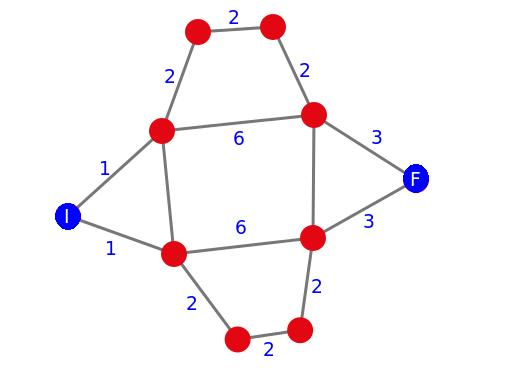
\includegraphics[scale=0.5]{./EJ3/grafoMultiCamino.jpeg}
 \\{$Grafo$ \ 3.2 - $Peor$ $Caso$}
  \end{center}
  \vspace*{0.3cm}

Veamos en detalle como se comportan el mejor y peor caso con respecto a la complejidad calculada.\\

  
  \vspace*{0.3cm} \vspace*{0.3cm}
  \begin{center}
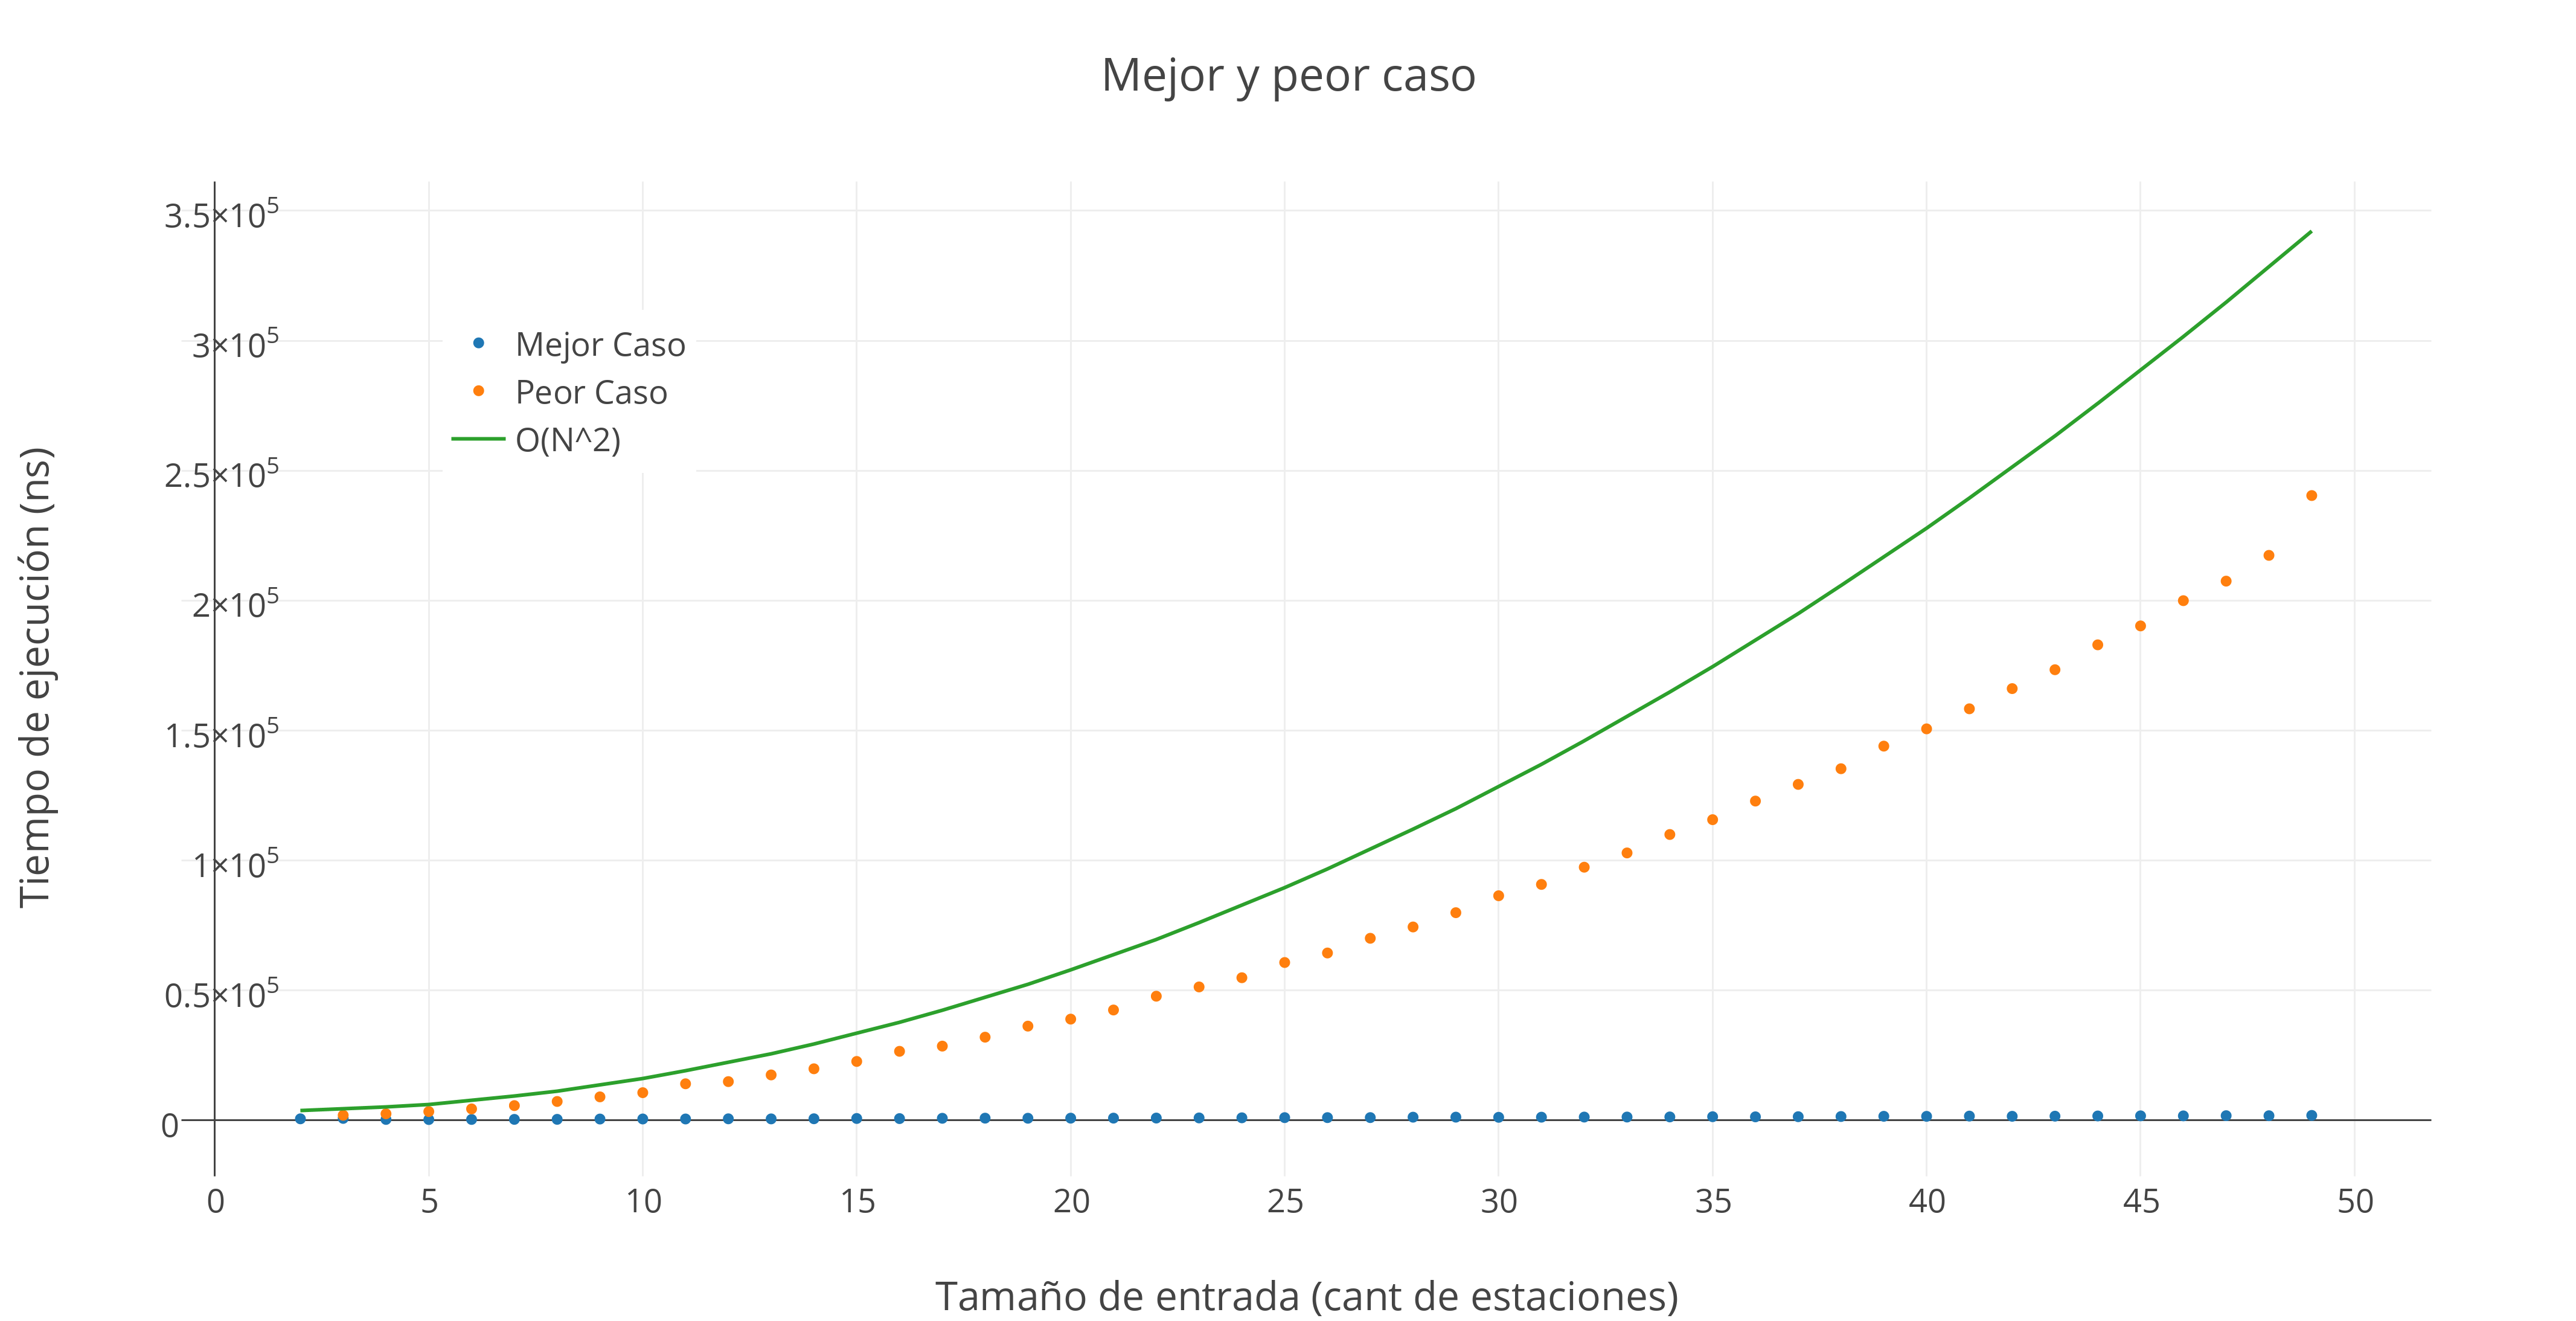
\includegraphics[scale=0.5]{./EJ3/mejorYpeorCaso.png}
{Gr\'afico 3.2 - $Comparativo$}
  \end{center}
  \vspace*{0.3cm}

Podemos ver en este gr\'afico comparativo como las familias est\'an acotadas por la funci\'on de la complejidad te\'orica calculada.\\
  
Dada la escala utilizada para el grafico 3.2 la funcion del mejor caso se torna constante, y no puede visualizarse correctamente, es por esto que desarrollamos otro gr\'afico para poder observar con mayor detenimiento dicha funci\'on y la misma ser\'a contrastada con la cota inferior.
  
  \vspace*{0.3cm} \vspace*{0.3cm}
  \begin{center}
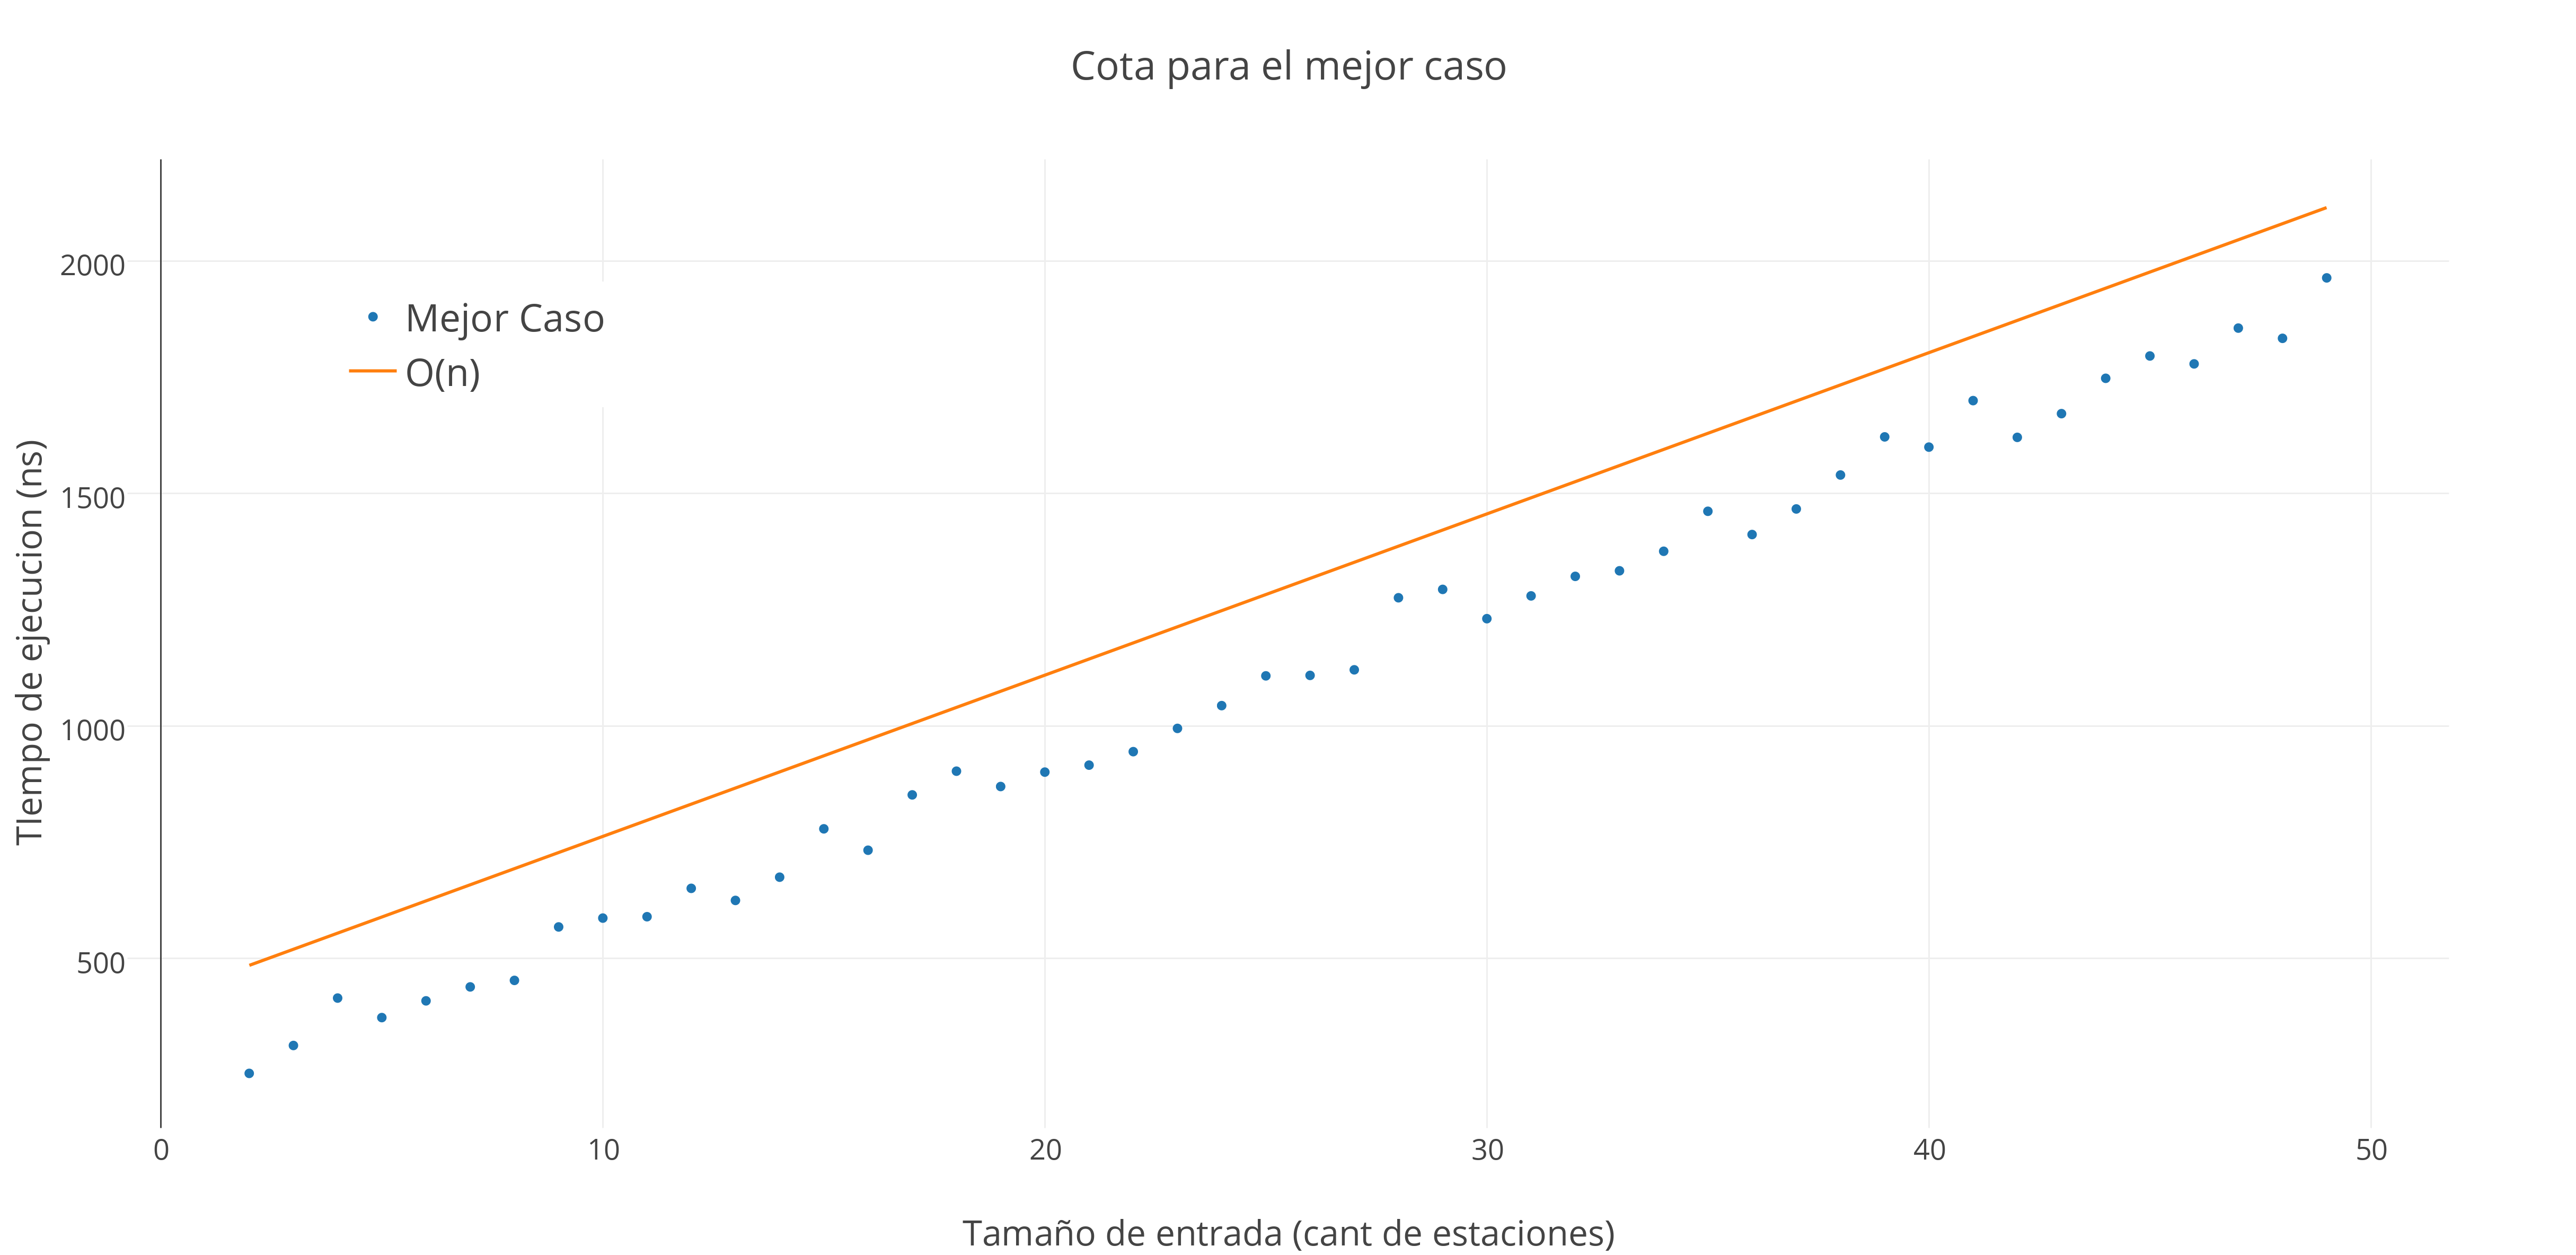
\includegraphics[scale=0.5]{./EJ3/Mejorcasoycotainferior.png}
{Gr\'afico 3.3 - \textit{Mejor caso contra cota inferior}}
  \end{center}
  \vspace*{0.3cm}

  
Luego de dichos experimentos y casos probados, se puede concluir que a pesar de tener ciclos en todas las salas y donde dichos ciclos presenten aristas con pesos iguales lo que generara al algoritmo la posibilidad de crear varias ramas posibles de soluci\'on nos mantenemos dentro de la complejidad propuesta como hab\'iamos mostrado en nuestro desarrollo de la complejidad.\\
